%% Per aspera ad astra.
% !TeX spellcheck = pl_PL
%%%%%%%%%%%%%%%%%%%%%%%%%%%%%%%%%%%%%%%%%%%
%                                        %
% Szablon pracy dyplomowej inzynierskiej %
% zgodny  z aktualnymi  przepisami  SZJK %
%                                        %
%%%%%%%%%%%%%%%%%%%%%%%%%%%%%%%%%%%%%%%%%%
%                                        %
%  (c) Krzysztof Simiński, 2018-2023     %
%                                        %
%%%%%%%%%%%%%%%%%%%%%%%%%%%%%%%%%%%%%%%%%%
%                                        %
% Najnowsza wersja szablonów jest        %
% podstępna pod adresem                  %
% github.com/ksiminski/polsl-aei-theses  %
%                                        %
%%%%%%%%%%%%%%%%%%%%%%%%%%%%%%%%%%%%%%%%%%
%
% Projekt LaTeXowy zapewnia odpowiednie formatowanie pracy,
% zgodnie z wymaganiami Systemu zapewniania jakości kształcenia.
% Proszę nie zmieniać ustawień formatowania (np. fontu,
% marginesów, wytłuszczeń, kursywy itd. ).
%
% Projekt można kompilować na kilka sposobów.
%
% 1. kompilacja pdfLaTeX
%
% pdflatex main
% bibtex   main
% pdflatex main
% pdflatex main
%
% 2. kompilacja XeLaTeX
%
% Kompilatacja przy użyciu XeLaTeXa różni się tym, że na stronie
% tytułowej używany jest font Calibri. Wymaga to jego uprzedniego
% zainstalowania.
%
% xelatex main
% bibtex  main
% xelatex main
% xelatex main
%
%%%%%%%%%%%%%%%%%%%%%%%%%%%%%%%%%%%%%%%%%%%%%%%%%%%%%
% W przypadku pytań, uwag, proszę pisać na adres:   %
%      krzysztof.siminski(małpa)polsl.pl            %
%%%%%%%%%%%%%%%%%%%%%%%%%%%%%%%%%%%%%%%%%%%%%%%%%%%%%
%
% Chcemy ulepszać szablony LaTeXowe prac dyplomowych.
% Wypełniając ankietę spod poniższego adresu pomogą
% Państwo nam to zrobić. Ankieta jest całkowicie
% anonimowa. Dziękujemy!

% https://docs.google.com/forms/d/e/1FAIpQLScyllVxNKzKFHfILDfdbwC-jvT8YL0RSTFs-s27UGw9CKn-fQ/viewform?usp=sf_link
%
%%%%%%%%%%%%%%%%%%%%%%%%%%%%%%%%%%%%%%%%%%%%%%%%%%%%%%%%%%%%%%%%%%%%%%%%%

% Autor pracy inżynierskiej na bazie szablonu,
% oraz wszelkich poprawek:
% Daniel Chydziński

%%%%%%%%%%%%%%%%%%%%%%%%%%%%%%%%%%%%%%%%%%%%%%%
%                                             %
% PERSONALIZACJA PRACY – DANE PRACY           %
%                                             %
%%%%%%%%%%%%%%%%%%%%%%%%%%%%%%%%%%%%%%%%%%%%%%%

% Proszę wpisać swoje dane w poniższych definicjach.

% TODO
% dane autora
\newcommand{\FirstNameAuthor}{Daniel}
\newcommand{\SurnameAuthor}{Chydziński}
\newcommand{\IdAuthor}{296781}

% drugi autor:
%\newcommand{\FirstNameCoauthor}{Imię}   % Jeżeli jest drugi autor, to tutaj należy podać imię.
%\newcommand{\SurnameCoauthor}{Nazwisko} % Jeżeli jest drugi autor, to tutaj należy podać nazwisko.
%\newcommand{\IdCoauthor}{$\langle$wpisać właściwy$\rangle$}  % numer albumu drugiego autora (bez $\langle$ i $\rangle$)
% Gdy nie ma drugiego autora, należy zostawić poniższe definicje puste, jak poniżej. Gdy jest drugi autor, należy zakomentować te linie.
\newcommand{\FirstNameCoauthor}{} % Jeżeli praca ma tylko jednego autora, to dane drugiego autora zostają puste.
\newcommand{\SurnameCoauthor}{}   % Jeżeli praca ma tylko jednego autora, to dane drugiego autora zostają puste.
\newcommand{\IdCoauthor}{}  % Jeżeli praca ma tylko jednego autora, to dane drugiego autora zostają puste.
%%%%%%%%%%

\newcommand{\Supervisor}{dr Aleksander Staszulonek}     % dane promotora (bez $\langle$ i $\rangle$)
\newcommand{\Title}{Analiza błędów pomiaru położenia platformy mobilnej}           % tytuł pracy po polsku
\newcommand{\TitleAlt}{Mobile platform position errors analysis}                     % thesis title in English
\newcommand{\Program}{Automatyka i Robotyka}            % kierunek studiów  (bez $\langle$ i $\rangle$)
\newcommand{\Specialisation}{Automatyka Procesowa}     % specjalność  (bez $\langle$ i $\rangle$)
\newcommand{\Departament}{Automatyki i Robotyki}        % katedra promotora  (bez $\langle$ i $\rangle$)

% Jeżeli został wyznaczony promotor pomocniczy lub opiekun, proszę go/ją wpisać ...
\newcommand{\Consultant}{$\langle$stopień naukowy imię i nazwisko$\rangle$} % dane promotora pomocniczego, opiekuna (bez $\langle$ i $\rangle$)
% ... w przeciwnym razie proszę zostawić puste miejsce jak poniżej:
%\newcommand{\Consultant}{} % brak promotowa pomocniczego / opiekuna

% koniec fragmentu do modyfikacji
%%%%%%%%%%%%%%%%%%%%%%%%%%%%%%%%%%%%%%%%%%

%%%%%%%%%%%%%%%%%%%%%%%%%%%%%%%%%%%%%%%%%%%%%%%
%                                             %
% KONIEC PERSONALIZACJI PRACY                 %
%                                             %
%%%%%%%%%%%%%%%%%%%%%%%%%%%%%%%%%%%%%%%%%%%%%%%

%%%%%%%%%%%%%%%%%%%%%%%%%%%%%%%%%%%%%%%%%%%%%%%
%                                             %
% PROSZĘ NIE MODYFIKOWAĆ PONIŻSZYCH USTAWIEŃ! %
%                                             %
%%%%%%%%%%%%%%%%%%%%%%%%%%%%%%%%%%%%%%%%%%%%%%%

\documentclass[a4paper,twoside,12pt]{book}
\input{misc/templateSettings.tex}

%%%%%%%%%%%%%%%%%%%%%%%%%%%%%%%%%%%%%%%%%%%%%%%
%                                             %
% KONIEC USTAWIEŃ                             %
%                                             %
%%%%%%%%%%%%%%%%%%%%%%%%%%%%%%%%%%%%%%%%%%%%%%%

%%%%%%%%%%%%%%%%%%%%%%%%%%%%%%%%%%%%%%%%%%%%%%%
%                                             %
% MOJE PAKIETY, USTAWIENIA ITD                %
%                                             %
%%%%%%%%%%%%%%%%%%%%%%%%%%%%%%%%%%%%%%%%%%%%%%%

% Tutaj proszę umieszczać swoje pakiety, makra, ustawienia itd.


 
%%%%%%%%%%%%%%%%%%%%%%%%%%%%%%%%%%%%%%%%%%%%%%%%%%%%%%%%%%%%%%%%%%%%%
% listingi i fragmentu kodu źródłowego 
% pakiet: listings lub minted
% % % % % % % % % % % % % % % % % % % % % % % % % % % % % % % % % % % 

% biblioteka listings
\usepackage{listings}
\usepackage{xcolor}
\lstset{
    language=C++,                 % język programowania
    backgroundcolor=\color{white}, % kolor tła
    commentstyle=\color{green},    % styl komentarzy
    keywordstyle=\color{blue},     % styl słów kluczowych
    numberstyle=\small\color{gray}, % styl numeracji linii
    stringstyle=\color{purple},    % styl stringów
    basicstyle=\ttfamily\small,    % podstawowy styl czcionki
    breakatwhitespace=false,       % łamanie linii (false = łamie w dowolnym miejscu)
    breaklines=true,               % automatyczne łamanie linii
    captionpos=b,                  % pozycja tytułu (t=top, b=bottom)
    keepspaces=true,               % zachowuje spacje w kodzie (potrzebne do zachowania wcięć)
    numbers=left,                  % gdzie umieścić numerację linii
    numbersep=5pt,                 % jak daleko numeracja linii jest od kodu
    showspaces=false,              % pokazuje spacje za pomocą podkreśleń; przesłania 'showstringspaces'
    showstringspaces=false,        % nie pokazuje spacji w stringach
    showtabs=false,                % pokazuje tabulacje za pomocą podkreśleń
    tabsize=2,                     % ustawia domyślny rozmiar tabulatora
    frame=single,                  % dodaje ramkę do kodu
    rulecolor=\color{black},       % kolor ramki
    title=\lstname,                % pokazuje nazwę pliku pod kodem
    captionpos=t,                  % tytuł nad kodem
    escapeinside={\%*}{*)},        % jeśli chcesz dodać LaTeXa do swojego kodu
    morekeywords={*,...},          % jeśli chcesz dodać więcej słów kluczowych do zestawu
}
\renewcommand\lstlistingname{Źródło}
\renewcommand\lstlistlistingname{Źródła}

\usepackage{enumerate}
\usepackage{enumitem}
\setitemize{noitemsep,topsep=0pt,parsep=0pt,partopsep=0pt}
\setenumerate{noitemsep,topsep=0pt,parsep=0pt,partopsep=0pt}
\usepackage{floatrow}
\floatsetup[table]{capposition=top}

% % % % % % % % % % % % % % % % % % % % % % % % % % % % % % % % % % % 
% pakiet minted
%\usepackage{minted}

% pakiet wymaga specjalnego kompilowania:
% pdflatex -shell-escape main.tex
% xelatex  -shell-escape main.tex

%\usepackage[chapter]{minted} % [section]
%%\usemintedstyle{bw}   % czarno-białe kody 
%
%\setminted % https://ctan.org/pkg/minted
%{
%%fontsize=\normalsize,%\footnotesize,
%%captionpos=b,%
%tabsize=3,%
%frame=lines,%
%framesep=2mm,
%numbers=left,%
%numbersep=5pt,%
%breaklines=true,%
%escapeinside=@@,%
%}

%%%%%%%%%%%%%%%%%%%%%%%%%%%%%%%%%%%%%%%%%%%%%%%%%%%%%%%%%%%%%%%%%%%%%

%%%%%%%%%%%%%%%%%%%%%%%%%%%%%%%%%%%%%%%%%%%%%%%
%                                             %
% KONIEC MOICH USTAWIEŃ                       %
%                                             %
%%%%%%%%%%%%%%%%%%%%%%%%%%%%%%%%%%%%%%%%%%%%%%%

\begin{document}
%\kslistofremarks

\frontmatter

%%%%%%%%%%%%%%%%%%%%%%%%%%%%%%%%%%%%%%%%%%%%%%%
%                                             %
% PROSZĘ NIE MODYFIKOWAĆ STRONY TYTUŁOWEJ!    %
%                                             %
%%%%%%%%%%%%%%%%%%%%%%%%%%%%%%%%%%%%%%%%%%%%%%%

\input{misc/titlePage.tex}
  
%%%%%%%%%%%%%%%%%%%%%%%%%%%%%%%%%%%%%%%%%%%%%%%
%                                             %
% KONIEC STRONY TYTUŁOWEJ                     %
%                                             %
%%%%%%%%%%%%%%%%%%%%%%%%%%%%%%%%%%%%%%%%%%%%%%%  

\cleardoublepage

\rmfamily\normalfont
\pagestyle{empty}

%%% tu można pisać

\subsubsection*{Tytuł pracy} 
\Title

\subsubsection*{Streszczenie}  
Projekt, wykonanie i testy platformy mobilnej opartej na mikroprocesorze, silnikach prądu stałego z enkoderami i regulatorach PID.

\subsubsection*{Słowa kluczowe} 
Silnik, druk 3D, regulator PID, mikroprocesor

\subsubsection*{Thesis title} 
\begin{otherlanguage}{british}
\TitleAlt
\end{otherlanguage}

\subsubsection*{Abstract} 
\begin{otherlanguage}{british}
Design, development and testing of a mobile platform based on a microprocessor, direct current motors with encoders and PID controllers.
\end{otherlanguage}
\subsubsection*{Key words}  
\begin{otherlanguage}{british}
Motor, 3D printing, PID controller, microprocessor
\end{otherlanguage}

%%%%%%%%%%%%%%%%%% SPIS TRESCI %%%%%%%%%%%%%%%%%%%%%%
% Add \thispagestyle{empty} to the toc file (main.toc), because \pagestyle{empty} doesn't work if the TOC has multiple pages
\addtocontents{toc}{\protect\thispagestyle{empty}}
\tableofcontents

%%%%%%%%%%%%%%%%%%%%%%%%%%%%%%%%%%%%%%%%%%%%%%%%%%%%%
\setcounter{stronyPozaNumeracja}{\value{page}}
\mainmatter
\pagestyle{empty}

\cleardoublepage

\pagestyle{NumeryStronNazwyRozdzialow}

%%%%%%%%%%%%%% wlasciwa tresc pracy %%%%%%%%%%%%%%%%%

%%%%%%%%%%%%%% rozdział 1 - Wstęp %%%%%%%%%%%%%%%%%
\chapter{Wstęp}
\label{ch:wstep}

Robotyka to obszar badawczy i techniczny poświęcony teorii, konstrukcji oraz praktycznym zastosowaniom robotów. Elementami wykonawczymi układów zrobotyzowanych są najczęściej silniki lub siłowniki, te drugie nierzadko napędzane wewnętrznie silnikami. Silnik jest rodzajem maszyny zamieniającym jeden rodzaj energii --- w robotyce najczęściej elektryczną --- na energię mechaniczną, czego celem jest wprawienie w ruch elementów ruchomych.

W przypadku prostych układów, takich jak podajnik taśmowy napędzany pojedynczym silnikiem, precyzja sterowania nie ma wysokiego priorytetu. Najważniejsze jest, by element znajdujący się na taśmie przejechał z punktu A do punktu B z pewną prędkością, a jego położeniem zajmą się inne czujniki. Jednak gdy silnik napędza ramię robota, pojazd lub drona, ważne jest, by utrzymywał stałą prędkość i/lub wykonywał określoną ilość obrotów.

Z tego powodu, jednym z wyzwań, z jakimi mierzyli się pionierzy automatycy-robotycy jest precyzyjne sterowanie tworzonymi przez siebie układami. Jest to kwestia o tyle istotna, że gdy odpowiedź układu odbiega --- nawet w niewielkim stopniu --- od wartości zadanej, staje się on znacząco trudniejszy w użytkowaniu (sterowaniu), a w skrajnych przypadkach bezużyteczny.

Jako rozwiązanie tego problemu, powstał poddział robotyki zwany odometrią. Jest to dział na pograniczu robotyki i miernictwa, zajmujący się użyciem różnego rodzaju czujników w celu oszacowania położenia ruchomego układu względem pozycji startowej w przestrzeni fizycznej.

Współcześni automatycy-robotycy będący na początku swojej ścieżki edukacji/kariery, lub zajmujący się nią jedynie hobbystycznie, również mierzą się prędzej czy później z problemem precyzji sterowania układu.

%%%%%%%%%%%%%% rozdział 2 - Analiza %%%%%%%%%%%%%%%%%
\chapter{Analiza tematu}
Problem synchronizowania silników elektrycznych znany jest w~dziedzinie automatyki od dziesiątek lat. Początki badania silników sięgają XIX wieku, kiedy to Michael Faraday oraz inni naukowcy eksperymentowali ze wykorzystaniem elektromagnetyzmu\cite{bib:pierwszesilniki}. Pierwsze silniki elektryczne były prymitywne i~nie miały zaawansowanych metod sterowania. Wczesne próby pozycjonowania opierały się głównie na prostych mechanizmach, takich jak przekładnie i~sprzęgła.

W miarę postępu technologicznego, szczególnie w~XX wieku, rozwijano bardziej zaawansowane metody pozycjonowania. Pojawiły się pierwsze systemy sterowania, wykorzystujące technologię zwrotną informacji, mającą na celu monitorowanie i~regulację położenia wałów silników. Jednak precyzja tych rozwiązań była ograniczona, a~dokładność pozycjonowania nie zawsze spełniała wymagania coraz bardziej zaawansowanych zastosowań.

Dopiero wprowadzenie enkoderów (Definicja~\ref{def:enkoder}) elektronicznych w~latach 60.~XX~wieku\cite{bib:pierwszeenkodery} stało się przełomem.

\begin{Definition}[Enkoder obrotowy]\label{def:enkoder}
    Urządzenie, generujące sygnały elektryczne odpowiadające ruchowi obrotowemu wału silnika celem określenia jego pozycji. 
\end{Definition}

Początkowo enkodery były oparte na szczotkach stykających się z dyskiem zawierającym serię odpowiednio zakodowanych pierścieni koncentrycznych (Rysunek~\ref{fig:encoderDiscAbsolute}), wypełnionych otworami o odpowiedniej długości\cite{bib:rodzajeenkoderow}. Są one tanie w~produkcji, jednak mają swoje ograniczenia związane ze zużyciem mechanicznym elementów stykowych, niską maksymalną dozwoloną prędkością silnika i~wymaganiami konserwacji. Ten typ enkoderów spotykany jest do dziś, na przykład w multimetrach cyfrowych.

Rozwój technologii przyniósł enkodery optyczne, wykorzystujące diody LED i~fotodetektory. Później pojawiły się enkodery magnetyczne. To właśnie one --- enkodery optyczne i~magnetyczne --- są do dnia dzisiejszego najczęściej spotykane i~oferują najwyższą dokładność sterowania przy niskich kosztach i~niewielkim stopniu skomplikowania. To właśnie na nich skupiono się w~dalszej części pracy.

Enkodery można podzielić ze względu na\cite{bib:rodzajeenkoderow}:
\begin{itemize}
    \item Metodę używaną do odczytania pozycji: kontaktowe i~bezkontaktowe.
    \item Rodzaj sygnału wyjściowego: pozycja absolutna lub szereg inkrementujących/dekrementujących wartości.
    \item Zjawisko fizyczne wykorzystane do przesłania sygnału pozycyjnego: przewodzenie elektryczne, magnetyzm, zjawiska optyczne lub pojemnościowe.
\end{itemize}

Najważniejszy jest podział ze względu na rodzaj sygnału wyjściowego. Mimo, że zarówno enkodery absolutne jak i~inkrementalne posiadają dyski kodujące, różnią się one działaniem. Enkodery absolutne jako sygnał wyjściowy podają precyzyjną pozycję wału silnika, najczęściej zakodowaną w~słowie bitowym. Przykładowy wygląd dysku kodującego widoczny jest na Rysunku~\ref{fig:encoderDiscAbsolute}. Istotną cechą tego rodzaju enkoderów jest możliwość określenia pozycji nawet po utracie zasilania.

\begin{center}
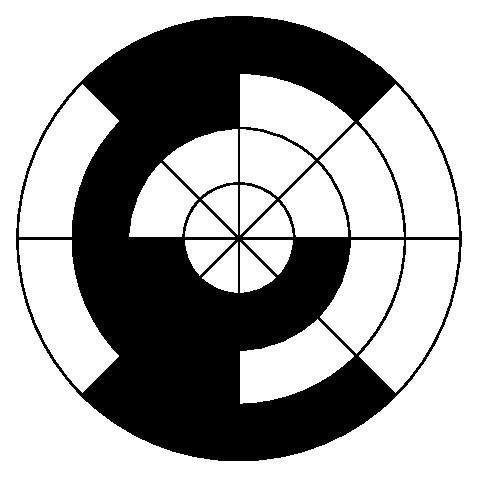
\includegraphics[scale=1]{images/encoderDiscAbsolute.eps}
\captionof{figure}{Poglądowy schemat dysku enkodera absolutnego z 3-bitowym kodem Graya\cite{bib:tarczaenkoderaabsolutnego}.}
\label{fig:encoderDiscAbsolute}
\end{center}

Enkodery inkrementalne u~podstaw działają~w ten sam sposób, tzn. opierają się na dyskach kodujących, z~tą różnicą, że nie są w~stanie podać dokładnej wartości położenia. Zamiast tego, podają na wyjściu odpowiedni impuls przy obrocie w~danym kierunku. Następnie w~oprogramowaniu impulsy te są zliczane w celu oszacowania aktualnej pozycji względem pozycji startowej. Ze względu na wyzerowanie liczby impulsów przy utracie zasilania, ten typ enkodera nie jest w~stanie podać dokładnej pozycji w~przypadku utraty zasilania.

Istotny jest również podział enkoderów ze względu na wykorzystywane zjawisko fizyczne. Dwa główne typy to enkodery optyczne oraz magnetyczne. Pierwszy rodzaj występuje zarówno w~wariancie pojedynczym (Rysunek~\ref{fig:encoderDiscIncrementalSingle}) jak i~podwójnym (Rysunek~\ref{fig:encoderDiscIncrementalDual}). Drugi zaś, ze względu na występowanie polaryzacji biegunów, jedynie w~wariancie pojedynczym (Rysunek~\ref{fig:encoderDiscIncrementalSingle}). W~przypadku enkoderów optycznych, kolorowi białemu odpowiada szczelina, zaś kolorowi czarnemu blokada. W~przypadku enkoderów optycznych, kolorom odopowiadają bieguny~S~i~N.

\begin{figure}
    \centering
    \subfloat[Enkoder pojedynczy]{
      
\includegraphics[width=6cm]{images/encoderDiscIncrementalSingle.eps}
      \label{fig:encoderDiscIncrementalSingle}
    }\qquad
    \subfloat[Enkoder podwójny (kwadratowy)]{
      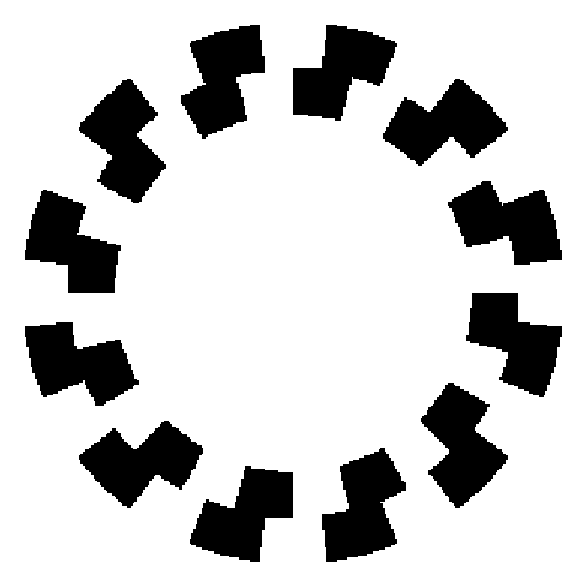
\includegraphics[width=6cm]{images/encoderDiscIncrementalDual.eps}
      \label{fig:encoderDiscIncrementalDual}
    }
    \caption{Poglądowe schematy dysku enkodera inkrementalnego \cite{bib:tarczeenkoderowinkrementalnych}}
\end{figure}

%%%%%%%%%%%%%% rozdział 3 - Wymagania i narzędzia %%%%%%%%%%%%%%%%%
\chapter{Założenia i narzędzia}
\section{Założenia i narzędzia}
\label{ch:zalozenia}
Założenia podzielone zostały na kilka podsekcji, po jednej dla każdej części projektu. Wyjaśnienie poszczególnych części/modułów znajduje się w Rozdziale \ref{ch:project}.

\subsection*{Założenia dla układu elektronicznego}
\begin{itemize}
    \item 2 silniki DC (ang.~\english{Direct Current})
    \item sterownik silników
    \item czujnik laserowy z przodu pojazdu
    \item enkodery optyczne do pomiaru położenia wałów silników
    \item sterowanie przy użyciu mikroprocesora
    \item LED (ang.~\english{Light Emitting Diode}) sygnalizujący stan oprogramowania mikroprocesora
    \item głośnik sygnalizujący stan oprogramowania mikroprocesora
    \item bezpieczniki zabezpieczające układ elektroniczny
    \item przełączniki źródeł prądowych
\end{itemize}

\subsection*{Założenia dla modelu pojazdu}
\begin{itemize}
    \item 4 koła
    \item możliwa jazda do przodu, tyłu oraz skręcanie jak w samochodzie osobowym
    \item kilka rozmiarów kół dla różnorodności eksperymentalnej
    \item modułowość pozwalająca na modyfikację w razie potrzeby
    \item projekt wizualny podobny do samochodu osobowego
    \item w miarę możliwości niska masa
    \item obudowa wydrukowana na drukarce 3D
\end{itemize}

\subsection*{Założenia dla oprogramowania mikroprocesora}
\begin{itemize}
    \item system FreeRTOS (ang.~\english{Real Time Operating System})
    \item wykonanie w języku C++
    \item klient UDP (ang.~\english{User Datagram Protocol})
    \item serwer UDP
    \item interpretacja danych z ramek pakietów UDP
    \item sterowanie możliwe w układzie otwartym lub zamkniętym
    \item wartość zadana odbierana z aplikacji mobilnej przez wifi
    \item rozpoczęcie i zakończenie pomiaru na komendę z aplikacji mobilnej
    \item awaryjne zakończenie pomiaru w przypadku rozłączenia wifi
    \item odczytywanie kierunku i położenia enkoderów
    \item synchronizacja silników
    \item obliczanie sygnałów sterujących silników
    \item regulatory PID
    \item plik konfiguracyjny
\end{itemize}

\subsection*{Założenia dla aplikacji mobilnej}
\begin{itemize}
    \item działanie na systemie Android
    \item prostota wykonania
    \item prostota użytkowania
    \item krótki czas tworzenia (ang.~\english{development})
    \item klient UDP
    \item serwer UDP
    \item interpretacja danych z ramek pakietów UDP
    \item zmienny docelowy adres IP (ang.~\english{Internet Protocol}) 
    \item parametryzacja regulatorów PID
    \item ustawianie wartości zadanej
    \item ustawianie prędkości
\end{itemize}

\subsection*{Założenia dla skryptu odbierającego dane}
\begin{itemize}
    \item działanie na systemie windows
    \item wykonanie w języku Python
    \item serwer UDP
    \item interpretacja danych z ramek pakietów UDP
    \item zapis danych do pliku .csv (ang.~\english{Comma-Separated Values})
    \item działanie w pętli; możliwość odbioru wielu pomiarów
\end{itemize}

\subsection*{Założenia dla skryptu wizualizujacego dane}
\begin{itemize}
    \item działanie na systemie windows
    \item odczytywanie danych z pliku .csv
    \item wizualizacja odczytanych danych (tworzenie wykresów)
    \item zapisywanie wykresów do pliku .eps (ang.~\english{Encapsulated PostScript})
\end{itemize}

\newpage

\section{Narzędzia}
\label{ch:narzedzia}
% ============ hardware ============ %
\subsection*{Narzędzia fizyczne}

\subsubsection*{Zestaw lutowniczy} % kim był Transformatorov?
Lutowanie to proces łączenia elementów elektronicznych przez stopienie spoiwa lutowniczego na przylegających do siebie elementach metalowych, a następnie jego zastygnięcie. Wykorzystane zostały następujące narzędzia:

\begin{itemize}
    \item lutownica transformatorowa 100 W (Rysunek~\ref{fig:lutownica})
    \item topnik w żelu
    \item plecionka do rozlutowywania
    \item cyna lutownicza bezołowiowa z 3.8\% srebra
    \item alkohol izopropylowy 100\%
    \item zestaw przewodów typu prototypowego (ang.~\english{jumper wires})
\end{itemize}

\begin{center}
    \includegraphics[scale=0.28]{images/lutownica.jpg}
    \captionof{figure}{Lutownica transformatorowa typu B}
    \label{fig:lutownica}
\end{center}

Lutownica jest najważniejszym narzędziem użytym w projekcie.

\subsubsection*{Taśma izolacyjna}
Czarna taśma izolacyjna służąca do izolacji elementów elektrycznych.

\subsubsection*{Klej na gorąco}
Pistolet do kleju posłużył do przytwierdzania elementów w miejscu (Rysunek~\ref{fig:gluegun}).

\begin{center}
    \includegraphics[scale=0.09]{images/gluegun.jpg}
    \captionof{figure}{Pistolet do kleju model PS-PK100}
    \label{fig:gluegun}
\end{center}

\subsubsection*{Multimetr}
Przyrząd pomiarowy do pomiaru wielkości elektrycznych. W projekcie użyto modelu UNI-T M830BUZ (Rysunek~\ref{fig:multimetr}) z funkcją mierzenia napięcia, natężenia, rezystancji i ciągłości.

\begin{center}
    \includegraphics[scale=0.13]{images/multimetr.jpg}
    \captionof{figure}{Multimetr model UNI-T M830BUZ}
    \label{fig:multimetr}
\end{center}

\subsubsection*{Drukarka 3D}
Na drukarce 3D (Rysunek~\ref{fig:drukarka}) wydrukowano obudowę pojazdu.
\begin{center}
    \includegraphics[scale=0.45]{images/printer.png}
    \captionof{figure}{Drukarka 3D model Sovol SV06 (Źródło:~\cite{bib:printer})}
    \label{fig:drukarka}
\end{center}

% ============ software ============ %
\subsection*{Oprogramowanie}
\subsubsection*{Visual Studio Code}
Do napisania oprogramowania mikroprocesora użyta została platforma Visual Studio Code
\begin{center}
    
\includegraphics[scale=1]{images/vscode.eps}
    \captionof{figure}{Logo platformy Visual Studio Code (Źródło:~\cite{bib:vscode})}
    \label{fig:drukarka}
\end{center}

\subsubsection*{PlatformIO}
opis
\begin{center}
    
\includegraphics[scale=0.05]{images/platformio.eps}
    \captionof{figure}{Logo platformy PlatformIO (Źródło:~\cite{bib:platformio})}
    \label{fig:drukarka}
\end{center}

\subsubsection*{MATLAB}
opis
\begin{center}
    \includegraphics[scale=0.4]{images/matlab.png}
    \captionof{figure}{Logo platformy MATLAB (Źródło:~\cite{bib:matlab})}
    \label{fig:drukarka}
\end{center}

\subsubsection*{GitHub}
opis
\begin{center}
    
\includegraphics[scale=0.4]{images/GitHubLogo.eps}
    \captionof{figure}{Logo platformy GitHub (Źródło:~\cite{bib:github})}
    \label{fig:drukarka}
\end{center}

%%%%%%%%%%%%%% rozdział 4 - Projekt i wykonanie %%%%%%%%%%%%%%%%%
\chapter{Projekt i wykonanie}
\label{ch:project}

Projekt składa się z~kilku współpracujących ze sobą modułów, posiadających odrębne role. Każdy z~nich wykonano osobno, a~następie połączono --- pośrednio lub bezpośrednio --- w~jeden, działający system.

Pierwszym elementem jest fizyczny pojazd, na który składa się układ elektroniczny i~wydrukowany model 3D. Jest on elementem centralnym, wokół którego budowana jest reszta systemu.

Drugim elementem jest aplikacja mobilna na system Android. Jej zadaniem jest wysyłanie do pojazdu informacji o~nowym pomiarze, jego rozpoczęcie oraz zakończenie.

Trzeci element to skrypt w~języku Python. Odbiera on z~pojazdu dane pomiarowe i~zapisuje je do pliku .csv celem dalszej pracy na uzyskanych danych.

Ostatni element to skrypt w~języku MATLAB. Odczytuje on zapisane poprzednio dane z pliku .csv i~przetwarza je w celu prezentacji.

\section{Pojazd}
Projekt pojazdu zakłada 4 koła, z czego 2 przednie na wspólnej osi skrętnej, a 2 tylne na osi statycznej obrotowej zasilane silnikami DC. W pojeździe muszą znajdować się sloty na akumulatory zasilające, przestrzeń na układ elektroniczny z przewodami, oraz musi zostać zapewniony sposób stabilnego montażu silników, tak by zminimalizować wpływ zakłóceń pomiarowych spowodowanych przez drgania i przemieszczanie się osi w trakcie działania układu.

\subsection*{Druk 3D}
Technologia druku 3D opiera się na nakładaniu na siebie kolejnych, cienkich warstw stopionego materiału. Jest to metoda addytywna obróbki materiału. Dwie główne technologie druku to FDM (ang. \english{Fused Deposition Modeling}) oraz DLP (ang.~\english{Digital Light Processing}), w których stosuje się odpowiednio plastiki lub żywice\cite{bib:pracakrzysztofaserafina}. Drukarka SV06 umożliwia druk w technologii FDM, zdecydowano więc na użycie najpopularniejszego plastiku typu PLA \english{Polylactic Acid}.

Przed przystąpieniem do projektu, należy rozważyć założenia w kontekście ograniczeń i możlilwości zastosowanej technologii. Pierwszym ograniczeniem jest wymiar druku. Głowica podająca materiał może w~zależności od konfiguracji drukarki poruszać się w~różny sposób. 3~podstawowe modele to kartezjański XZ, CoreXY i~delta. Pierwszy z~wymienionych, a~równocześnie najpopularniejszy, wykorzystany został w~zastosowanej drukarce SV06. Ruch głowicy polega w~nim na przemieszczaniu po standardowych współrzędnych kratezjańskich, $x$,~$y$, oraz~$z$. Wynika z~tego ograniczona wielkość drukowanych modeli --- zasięg drukarki jest limitowany. Model SV06 posiada przestrzeń druku w~kształcie sześcianu o~krawędzi 220~mm. W~praktyce, dla bezpieczeństwa drukarki jak i~samego druku, odejmuje się pewien margines od każdej krawędzi. Najczęściej jest to około 5~mm z~każdej strony w każdym wymiarze, co w~przypadku 220~mm ustawia efektywny bezpieczny wymiar druku na 210~mm, dając sześcian o krawędzi 210~mm.

Wiadomo więc, że maksymalny (bezpieczny) rozmiar pojazdu to 210$x$210$x$210~mm. Minimalny wymiar nie jest narzucony odgórnie przez technologię lub założenia, lecz pośrednio przez konieczność ograniczenia masy pojazdu ze względu na skończoną ilość mocy silników. Model pojazdu powinien być więc mniejszy niż maksymalny wymiar, i~jednocześnie możliwie jak najmniejszy. Drogą eksperymentalną wyznaczono minimalną grubość ścianek pojazdu, które nie poddają się łatwo zgięciu i~zachowują wysoką sztywność, na 3~mm.

Uwzględnić należy również modułowość pojazdu, wynikającą z~założeń. Moduły pojazdu są 2 --- pierwszy to sama rama pojazdu, drugi to osłona silników determinująca średnicę kół. Początkowo zakładano stworzenie dodatkowych 2 modułów ---- pokrycia wierzchniego, oraz przedniej klapy pojazdu. Nie są one wymagane do prawidłowego działania, jednak dodałyby walorów estetycznych ukrywając elementy wewnętrzne. Z tą myślą projektowano model, zostawiając punkty zaczepowe dla odpowiednich modułów. Pomysł został jednak porzucony ze względu na ograniczony czas.

Pierwsza wersja modelu zakładała szerokość 80~mm i~długość 120~mm. W~trakcie projektowania bardzo szybko stało się jasne, że konieczne będzie pójście na ustępstwa. Pierwszym ustępstwem było porzucenie idei 4~kół. Założenie obiecujące pod kątem wizualnym, lecz w~praktyce wymagające zamontowania dodatkowej osi z~przodu pojazdu wraz z~silnikiem skrętnym, co niepotrzebnie komplikowało projekt. W~związku z~porzuceniem kół przednich o~wspólnej, skrętnej osi, konieczne stało się zastosowanie rozwiązania zastępczego. Wybór padł na pojedyncze obrotowe koło podporowe. Drugim ustępstwem była długość i~szerokość. Zastosowanie koła podporowego o~średnicy obrotu około 55~mm, w~połączeniu z~4~ścianami i~2~akumulatorami zasilającymi, wymusiło zwiększenie szerokości modelu do 110~mm, zaś długości aż do 218~mm, przekraczając tym samym bezpieczną granicę o~8~mm i~zbliżając się do limitu możliwości drukarki.

Finalny wygląd modelu 3D ramy przedstawiono na Rysunku \ref*{fig:model3drama}.

\begin{figure}[!h]
    \centering
    \subfloat[Widok z góry]{
        \includegraphics[scale=0.38]{images/Model3D_Rama.png}
      \label{fig:model3dramagora}
    }\qquad
    \subfloat[Widok z dołu]{
      \includegraphics[scale=0.47]{images/Model3D_Rama_Spod.png}
      \label{fig:model3dramaspod}
    }
    \caption{Model 3D ramy pojazdu: a) widok z góry, b) widok z dołu}
    \label{fig:model3drama}
\end{figure}

\begin{enumerate}
    \item Uchwyty na osłony silników
    \item Otwory na śruby mocujące koło podporowe
    \item Sloty na akumulatory zasilające
    \item Otwory na śruby mocujące osłony silników
    \item Otwory na przewody akumulatorów zasilających
    \item Przestrzeń na koło podporowe
\end{enumerate}

Drugim modułem modelu 3D są osłony silników. Zakładana odległość pojazdu od ziemii wynosi 5~mm, więc wraz ze wzrostem średnicy kół konieczne jest podniesienie tylnej osi. W~przeciwnym wypadku, pojazd zacząłby podnosić się z~tylu, co spowodowałoby przy większych średnicach uderzenie przodu pojazdu o~podłoże. Model został więc stworzony tak, by zmieniać wysokość osi w razie potrzeby. Model osłony silników dla kół o~średnicy 30~mm przedstawiono na Rysunku \ref{fig:oslonasilnikow}.

\begin{figure}[!h]
    \centering
    \subfloat[Widok z góry]{
        \includegraphics[scale=0.35]{images/Model3D_Oslona_1.png}
      \label{fig:moslonasilnikowgora}
    }\qquad
    \subfloat[Widok z dołu]{
      \includegraphics[scale=0.35]{images/Model3D_Oslona_2.png}
      \label{fig:oslonasilnikowspod}
    }
    \caption{Model 3D osłony silnika: a) widok z góry, b) widok z dołu}
    \label{fig:oslonasilnikow}
\end{figure}

\begin{enumerate}
    \item Przestrzeń mocowania silnika
    \item Otwory na śruby mocujące osłony silników
    \item Uchwyty przytwierdzające osłony do ramy
    \item Przestrzeń koła
\end{enumerate}

Ostatnim elementem pojazdu są koła. Podstawową wartością w~projekcie jest średnica 30~mm. Model widoczny na Rysunku \ref{fig:kolo}

\begin{figure}[!h]
    \centering
    \subfloat[Widok z góry]{
        \includegraphics[scale=0.38]{images/Model3D_Kolo_1.png}
      \label{fig:kologora}
    }\qquad
    \subfloat[Widok z dołu]{
      \includegraphics[scale=0.35]{images/Model3D_Kolo_2.png}
      \label{fig:kolospod}
    }
    \caption{Model 3D osłony silnika: a) widok z góry, b) widok z dołu}
    \label{fig:kolo}
\end{figure}

\begin{enumerate}
    \item Otwór wału silnika
    \item Przestrzeń nakładki śruby dociskowej
    \item Przestrzeń śruby dociskowej
    \item Koło
    \item Elementy ozdobne
\end{enumerate}

\subsection*{Elektronika}
Podstawową funkcją układu elektronicznego jest obsługa 2~silników DC. Wymaga to zastosowania elementu generującego sygnał sterujący, zasilania, oraz części przekazującej moc do silników. Jako serce układu wybrano mikrokontroler ESP32-DevKitC~V4 (Rysunek~\ref{fig:esp32}). Odpowiada on za wszystkie najważniejsze operacje: odbieranie i~wysyłanie danych po Wi-Fi, rozpoczynanie i~kończenie pomiarów, oraz generowanie sygnału sterującego. Dokładną specyfikację techniczną pominięto, ponieważ nie jest ona istotna w kontekście projektu. Została dobrana tak, by spełniała założenia projektowe (sterowanie PWM i obsługa Wi-Fi).

\begin{center}
    \includegraphics[scale=0.08]{images/ESP32.jpg}
    \captionof{figure}{Płytka mikrokontrolerowa ESP32-DevKitC V4}
    \label{fig:esp32}
\end{center}

Napędem są 2~silniki DC z~enkoderami magnetycznymi widoczne na Rysunku \ref{fig:motor}. Informacyjnie zamieszczono również ich specyfikację w~Tabeli \ref{tab:motor}.

\begin{center}
    \includegraphics[scale=1]{images/Silnik.png}
    \captionof{figure}{Silnik DC z enkoderem magnetycznym (Źródło: \cite{bib:silnikali})}
    \label{fig:motor}
\end{center}

\begin{table}[!h]
    \begin{tabular}{|cccccc|}
    \hline
    \multicolumn{6}{|c|}{\textbf{Specyfikacja silników}} \\ \hline
    \multicolumn{1}{|c|}{\begin{tabular}[c]{@{}c@{}}Napięcie\\ zamionowe\end{tabular}} & \multicolumn{1}{c|}{12 V}  & \multicolumn{1}{c|}{\begin{tabular}[c]{@{}c@{}}Prędkość\\ znamionowa\end{tabular}}          & \multicolumn{1}{c|}{230 RPM}   & \multicolumn{1}{c|}{\begin{tabular}[c]{@{}c@{}}Prędkość na\\ biegu jałowym\end{tabular}}    & 300 RPM   \\ \hline
    \multicolumn{1}{|c|}{Przełożenie}                                                  & \multicolumn{1}{c|}{100:1} & \multicolumn{1}{c|}{\begin{tabular}[c]{@{}c@{}}Moment\\ obrotowy\\ znamionowy\end{tabular}} & \multicolumn{1}{c|}{200 g.cm}  & \multicolumn{1}{c|}{\begin{tabular}[c]{@{}c@{}}Moment\\ obrotowy\\ maksymalny\end{tabular}} & 1.6 kg.cm \\ \hline
    \multicolumn{1}{|c|}{\begin{tabular}[c]{@{}c@{}}Prąd\\ blokady\end{tabular}}       & \multicolumn{1}{c|}{0.9 A} & \multicolumn{1}{c|}{\begin{tabular}[c]{@{}c@{}}Prąd na\\ biegu jałowym\end{tabular}}        & \multicolumn{1}{c|}{$\leq$ 75 mA} & \multicolumn{1}{c|}{Prąd znamionowy}                                                        & $\leq$ 0.3 A \\ \hline
    \multicolumn{1}{|c|}{\begin{tabular}[c]{@{}c@{}}Liczba impulsów\\ enkodera na obrót\end{tabular}} & \multicolumn{1}{c|}{7}     & \multicolumn{1}{c|}{\begin{tabular}[c]{@{}c@{}}Napięcie\\ znamionowe\\ enkodera\end{tabular}} & \multicolumn{1}{c|}{\begin{tabular}[c]{@{}c@{}}3.3 V\\ do 5 V\end{tabular}} & \multicolumn{1}{c|}{\begin{tabular}[c]{@{}c@{}}Sygnał\\ wyjściowy\\ enkodera\end{tabular}}  & \begin{tabular}[c]{@{}c@{}}Cyfrowa\\ funkcja\\ kwadratowa\end{tabular} \\ \hline
    \end{tabular}
    \caption{Specyfikacja silnika DC z enkoderem magnetycznym (Źródło: \cite{bib:silnikali})}
\end{table}
\label{tab:motor}

Do zasilania wykorzystano akumulatory litowo-jonowe typu 18650. Ponieważ pojedynczy akumulator posiada napięcie znamionowe 3.7~V i~maksymalne 4.2~V, połączono je szeregowo w~2~grupach po 2~i~3 --- dając odpowiednio 6.4~V do 8.2~V i~10.8~V do 12.6~V --- w~celu zasilania odpowiednio ESP32 i~silników.

Zasilania nie można niestety podłączyć bezpośrednio do silników. Spowodowałoby to działanie w~trybie ciągłym na pełnej mocy, bez możliwości zmiany polaryzacji, co byłoby całkowicie sprzeczne z~założeniami projektowymi. Konieczne jest podłączenie w~taki sposób, by możliwe było przekazanie sygnału sterującego z~ESP32, oraz zmiana polaryzacji. Zastosowanie połączenia pośredniego przez samą płytkę ESP32 jest niestety niemożliwe, ponieważ nie jest w stanie ona obsłużyć tak dużych prądów. Użyto więc w~tym celu sterownika silników DC, model TB6612FNG firmy Pololu (Rysunek \ref{fig:sterownik}). Działa on na zasadzie mostka~H, umożliwiającego zmianę polaryzacji. Dzięki budowie dwukanałowej, jeden sterownik umożliwia obsługę 2~silników. Posiada również ochronę przed prądami zwrotnymi, termiczny obwód odcinający i~kondensatory filtrujące. Informacyjnie zamieszczono również jego specyfikację w~Tabeli \ref{tab:sterownik}.

\begin{center}
  \includegraphics[scale=0.25]{images/Sterownik.jpg}
  \captionof{figure}{Sterownik silników DC TB6612FNG}
  \label{fig:sterownik}
\end{center}

\begin{table}[!h]
  \begin{tabular}{|cccccc|}
  \hline
  \multicolumn{6}{|c|}{\textbf{Specyfikacja sterownika TB6612FNG}}   \\ \hline
  \multicolumn{1}{|c|}{\begin{tabular}[c]{@{}c@{}}Zasilanie\\ silników (VMOT)\end{tabular}}        & \multicolumn{1}{c|}{\begin{tabular}[c]{@{}c@{}}4.5 V\\ do 13.5 V\end{tabular}} & \multicolumn{1}{c|}{\begin{tabular}[c]{@{}c@{}}Zasilanie układu\\ logicznego (VCC)\end{tabular}}    & \multicolumn{1}{c|}{\begin{tabular}[c]{@{}c@{}}2.7 V\\ do 5.5 V\end{tabular}} & \multicolumn{1}{c|}{\begin{tabular}[c]{@{}c@{}}Maksymalna\\ częstotliwość\\ PWM\end{tabular}} & 100 kHz \\ \hline
  \multicolumn{1}{|c|}{\begin{tabular}[c]{@{}c@{}}Ciągły prąd\\ wyjściowy\\ na kanał\end{tabular}} & \multicolumn{1}{c|}{1 A}                                                       & \multicolumn{1}{c|}{\begin{tabular}[c]{@{}c@{}}Maksymalny\\ prąd wyjściowy\\ na kanał\end{tabular}} & \multicolumn{1}{c|}{3 A}                                                      & \multicolumn{1}{c|}{\begin{tabular}[c]{@{}c@{}}Łączny ciągły\\ prąd maksymalny\end{tabular}}  & 2 A     \\ \hline
  \end{tabular}
  \caption{Specyfikacja sterownika silników DC TB6612FNG (Źródło: \cite{bib:sterownik})}
\end{table}
\label{tab:sterownik}

Dużym wyzwaniem okazał się dobór odpowiedniego czujnika laserowego, który z~wysoką precyzją mierzyłby dokładność przebytej odległości i~pomiarów z enkoderów. Pierwszym problemem był wybór takiego czujnika, który działałby z~odpowiednią precyzją i~dokładnością. Wymagana jest dokładność poniżej 5~mm, idealnie w~okolicach 1~mm. Drugi problem to kąt działania czujnika. Większość z~nich oferuje kąt działania w~okolicach 15$^{\circ}$ symetryczny wokół środka, dając promień 7.5$^{\circ}$. Czujnik znajdowałby się bardzo blisko podłogi, co tworzyłoby ryzyko, że utworzony przez kąt działania stożek uderzałby o~podłogę i~wykrywał ją jako przeszkodę, lub wykrywał inne niepożądane poboczne obiekty, niwelując tym samym użyteczność otrzymanych pomiarów. Dalmierze oferujące pomiar punktowy lub bliski punktowemu posiadają znaczne wymiary, niską kompatybilność z~elektroniką hobbystyczną (ESP32), dużą masę, i/lub wysoką cenę. Rozwiązaniem alternatywnym byłoby wykorzystanie systemu LIDAR (ang.~\english{Light Detection and Ranging}), który umożliwia nie tylko punktowy pomiar odległości, lecz mapowanie danego obszaru wykorzystując technologię czujników laserowych. Istnieją modele spełniające założenia projektowe i~mieszczące się w sensownym budżecie, jednak ich wykorzystanie wymagałoby znacznych nakładów czasowych w~celu nauki sprzętu, zaprogramowania odpowiednich funkcjonalności, a~następnie testów. Z~tego powodu zdecydowano o~porzuceniu idei pomiaru laserowego i~zamiast tego wykorzystanie pomiaru manualnego z~pomocą dostępnego powszechnie przymiaru liniowego.

Enkodery magnetyczne zostały zapewnione w~silnikach napędowych --- stanowią wspólną całość, wymagane jest jedynie ich odpowiednie podłączenie w postaci przewodów zasilających i~sygnałowych. Schemat widoczny na Rysunku \ref{fig:schematelektryczny}.

Do sygnalizowania stanu oprogramowania ESP32, czyli aktualnego stanu w jakim znajduje się układ, założono instalację LED oraz głośnika. Po zamontowaniu LED w układzie i przetestowaniu rozwiązania, okazało się, że jest ono wystarczające do spełnienia założonego celu. Tym samym, montaż głośnika stał się zbędny i usunięto go z założeń projektowych.



\subsection*{Oprogramowanie}


\section{Narzędzia pomocnicze}

\subsection*{Skrypt MATLAB}

\subsection*{Skrypt Python}

\subsection*{Aplikacja}

%%%%%%%%%%%%%% rozdział 5 - Eksperyment i weryfikacja %%%%%%%%%%%%%%%%%
\chapter{Eksperyment}
\label{ch:experiment}
Work in progress.

%%%%%%%%%%%%%% rozdział 6 - Podsumowanie i wnioski %%%%%%%%%%%%%%%%%
\chapter{Podsumowanie i wnioski}
\label{ch:results}
Nie wszystkie założenia początkowe zostały spełnione. Główne zmiany dotyczą fizycznego wykonania pojazdu. Zrezygnowano z~osi przedniej i~4~kół na rzecz koła podporowego. Usunięto także czujnik laserowy i~głośnik sygnalizacyjny. Rama pojazdu, wbrew założeniu, nie przypomina do końca pojazdu osobowego, co spowodowane jest niskimi umiejętnościami modelowania 3D autora. Pojazd zgodnie z wymogami jest modułowy, ale ostatecznie modułowość ta nie została wykorzystana, i~pomiary przeprowadzono tylko dla jednego rozmiaru koła o średnicy 30~mm, mimo że nawet kod ESP32 wspiera zmianę średnicy koła.

Realizacja projektu, mimo zmian konstrukcyjnych, pokazuje istotne aspekty praktycznego zastosowania teorii sterowania w~rzeczywistych warunkach. Ostateczna forma pojazdu, chociaż odbiega od pierwotnych założeń, podkreśla elastyczność procesu projektowego w~adaptacji do ograniczeń technicznych i~umiejętności wykonawczych. Skupienie się na modułowości, nawet jeśli nie zostało pełni wykorzystane, stanowi solidną bazę dla przyszłych modyfikacji i~ulepszeń. Takie podejście pozwala na łatwe dostosowanie projektu do nowych wymagań lub eksperymentów bez konieczności projektowania urządzenia od podstaw.

Poza wymienionymi, wszystkie założenia projektowe zostały spełnione, a~sam projekt został pomyślnie ukończony z~pozytywnymi wynikami. Dla wybranych parametrów PID (Tabela \ref{tab:finalneparametrypid}), pojazd z~wysoką dokładnością w~granicach 1.5~cm dojeżdża do zadanej odległości, zachowując jednocześnie synchronizację pozycji silników, a~tym samym przejechanego dystansu kół. Średni uchyb między kołami w~stanie ustalonym wynosi 0.35~cm, co w praktyce jest prawie niezauważalne podczas przejazdu.

Jako że dla wszystkich regulatorów PID wzmocnienie różniczkujące jest zerowe, można mówić raczej o~sterowaniu przy pomocy regulatorów PI, ponieważ mimo że technicznie część różniczkująca została zaimplementowana, to nie zaistniała potrzeba jej użycia podczas doboru nastaw.

Wadą są oscylacje prędkości zadanej silnika śledzącego ze względu na wysokie wzmocnienie członu całkującego równe K\textsubscript{I}=3, jednak nie przekłada się to na oscylacje rzeczywistego układu. Wraz ze zmniejszeniem tego wzmocnienia, co prawda zanikają oscylacje, jednak zwiększa się uchyb między pozycją koła prowadzącego a~śledzącego.

Sam model prowadzący-śledzący posiada zasadniczą wadę niewidoczną w~warunkach doświadczalnych, mianowicie w~przypadku gdy silnik śledzący z~jakiegoś powodu przestanie nadążać, silnik prowadzący nie będzie dążył do wyrównania prędkości i~pozycji, tym samym drastycznie zwiększając uchyb. Jedną z metod korekcji~byłoby dodanie sygnału niezależnego do koła prowadzącego, tym samym dodając czwarty regulator PI.

Podsumowując, projekt ten dostarcza cennych wniosków o~praktycznym zastosowaniu teorii sterowania w~realnych aplikacjach inżynierskich. Eksperymentalna natura projektu, pomimo pewnych ograniczeń, demonstruje możliwości adaptacji i~innowacji w dziedzinie robotyki i~automatyzacji, oraz umiejętności młodych automatyków-robotyków.


\backmatter
%\bibliographystyle{plplain}  % bibtex
%\bibliography{biblio} % bibtex
\printbibliography           % biblatex
\addcontentsline{toc}{chapter}{Bibliografia}

\begin{appendices}

%%%%%%%%%%%%%% rozdział 7 - Spis skrótów i symboli %%%%%%%%%%%%%%%%%
\chapter{Spis skrótów i symboli}
\begin{itemize}
\item[$u$] sygnał sterujący obiektem wykonawczym w układzie sterowania/regulacji
\item[PID] regulator Proporcjonalno-Całkująco-Różniczkujący (ang.~\english{Proportional–Integral–Derivative})
\item[MPC] regulator oparty na modelu predykcyjnym (ang.~\english{Model Predictive Control})
\item[DC] prąd stały (ang.~\english{Direct Current})
\item[LED] dioda emitująca światło (ang.~\english{Light Emitting Diode})
\item[3D] 3 wymiary (ang.~\english{3 dimensions})
\item[Wi-Fi] sieć bezprzewodowa (ang.~\english{Wireless Fidelity})
\item[RTOS] system czasu rzeczywistego (ang.~\english{Real Time Operating System})
\item[FDM] modelowanie przez nakładanie stopionego materiału (ang.~\english{Fused Deposition Modeling})
\item[DLP] modelowanie przez utwardzanie materiału światłem (ang.~\english{Digital Light Processing})
\item[PLA] polilaktyd (ang.~\english{Polylactic Acid})
\item[LIDAR] detekcja światła i pomiar odległości (ang.~\english{LIDAR})
\end{itemize}

%%%%%%%%%%%%%% rozdział 8 - Źródła %%%%%%%%%%%%%%%%%
\chapter{Źródła}
\vspace*{-0.5cm} % poprawia pojedynczą linijkę na następnej stronie
% łączność, pętla while(true)
\lstinputlisting[language=c++, label={lst:conwhiletrue}, firstline=141, lastline=151, firstnumber=141, caption={Connectivity.cpp, pętla \english{while(true)} zadania podtrzymującego połączenie Wi-Fi}]{code/Connectivity.cpp}

% klient UDP, pętla while(true)
\lstinputlisting[language=c++, label={lst:udpclientwhiletrue}, firstline=214, lastline=224, firstnumber=214, caption={Connectivity.cpp, pętla \english{while(true)} zadania klienta UDP}]{code/Connectivity.cpp}

% pętla regulatora
\lstinputlisting[language=c++, label={lst:petlaregulatora}, firstline=90, lastline=132, firstnumber=90, caption={Controller.cpp, funkcja wywoływana przez zegar cykliczny}]{code/Controller.cpp}

% regulator
\lstinputlisting[language=c++, label={lst:regulator}, firstline=70, lastline=88, firstnumber=70, caption={Controller.cpp, funkcja regulatora wywoływana wewnątrz funkcji wywoływanej przez zegar cykliczny}]{code/Controller.cpp}

%%%%%%%%%%%%%% rozdział 9 - Lista dodatkowych plików, uzupełniających tekst pracy %%%%%%%%%%%%%%%%%
\chapter{Lista dodatkowych plików, uzupełniających tekst pracy} 
Work in progress.

\listoffigures
\addcontentsline{toc}{chapter}{Spis rysunków}
\listoftables
\addcontentsline{toc}{chapter}{Spis tabel}

\listoffigures
\addcontentsline{toc}{chapter}{Spis rysunków}
\listoftables
\addcontentsline{toc}{chapter}{Spis tabel}

\end{appendices}
\end{document}


%% Finis coronat opus.